\chapter{O Script do Câncer de Mama}
\label{chapter:o_script_do_cancer_de_mama}


Não foi exposto aqui o código final inteiro, por ser bastante extenso, encontra-se ao final do trabalho no apêndice \ref{app:code}, seção
\ref{lst:code}, página \pageref{lst:code}, para quem se interessar, ler melhor.

As funções que se referem ao aprendizado de máquina são a parte principal do código e onde pode haver dúvidas quanto a sintaxe.
Portanto será explicado na seção \ref{sintaxe}.

Para executar o script, precisa ter o python \cite{PYTHON} instalado,
e então salvar o conteúdo do código no apêndice \ref{app:code} em um arquivo, por exemplo ``script.py'',
e colocar na mesma pasta do arquivo com o banco de dados
(\url{https://www.kaggle.com/uciml/breast-cancer-wisconsin-data/download}) \cite{BREASTCANCER}.
Em seguida, no local onde estão os arquivos executa-se:

\begin{lstlisting}[language=Python, caption=Executar Script.py]
python script.py
\end{lstlisting}

\section{Validação Cruzada}

Antes de ir diretamente ao código, é necessário a compreensão da validação cruzada.
A validação cruzada é um método de aprendizado de máquina em que utiliza-se uma
porcentagem para teste e outra para treinamento, comumente $10\%$ para testes e $90\%$ para treinamento.
Desta forma o script treina de diferentes formas melhorando sua confiabilidade.


Por exemplo, na figura \ref{fig:crossvalidation}, a base de dados foi dividida em 6,
e em cada iteração usa-se uma parte diferente como teste, e o restante para o treinamento.

\begin{figure}[H]
\begin{center}
\caption{Validação Cruzada}
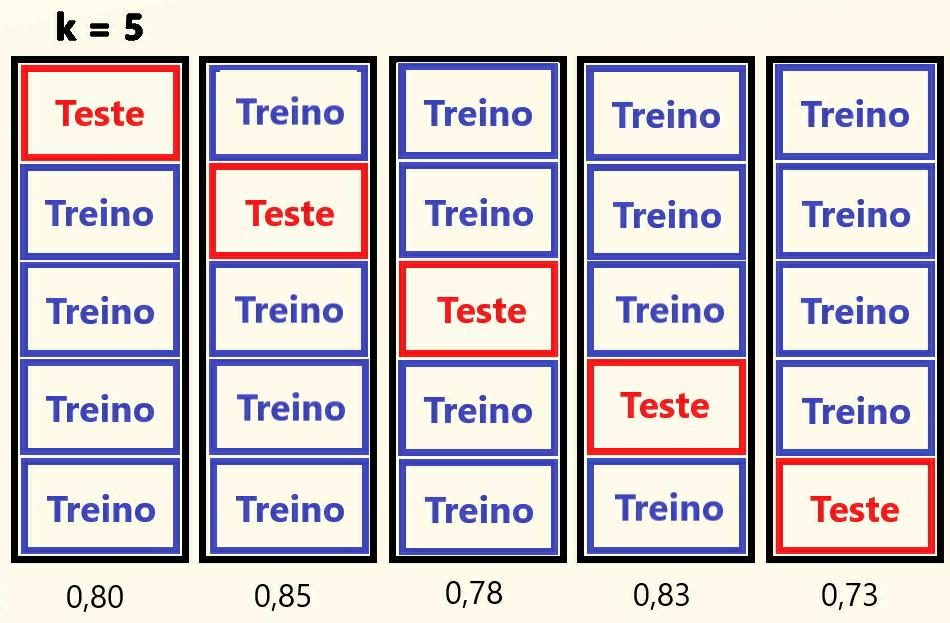
\includegraphics[width=12cm]{crossvalidation}
\label{fig:crossvalidation}
\end{center}
\legend{Fonte: \url{https://didatica.tech/wp-content/uploads/2019/10/Kfold_Resultados.png} \cite{CROSSVALIDATION} }
\end{figure}

\section{Sintaxe}
\label{sintaxe}
Primeiramente será explicada a função ``Máquina de Vetor de Suporte'',
ela é chamada na primeira linha do código \ref{alg:simples}.

Na segunda linha é chamada a validação cruzada $cros\_val\_score$ que salva na variável $scores$ um vetor com a acurácia das $10$ iterações.
Na terceira e quarta linha, informa na tela a média dos valores das acurácias.
A quinta, sexta e sétima servem para ao final do script, informar qual foi a função com o melhor desempenho.

\begin{lstlisting}[language=Python, caption=Sintaxe Simples, label=alg:simples]
svm = SVC(kernel='poly',degree=1)
scores = cross_val_score(svm, X, y, cv=10, scoring='accuracy')
function_print = 'SuppotVectorMachine:\t' + str(scores.mean())
print(function_print)
if scores.mean() > best_score:
  best_score = scores.mean()
  best_function=function_print
\end{lstlisting}

Por último será mostrada a função ``Árvore de decisão'' no código \ref{alg:parametro},
pois ela possui um parâmetro $max\_depth=n$ que pode variar,
e deseja-se saber para qual $n$ ela consegue a melhor acurácia.

Para isso o $n$ será variado de $1$ a $9$, como mostra as linhas $1$ e $2$.
As linhas $5$, $6$ e $7$ salvam o $n$ com a maior acurácia juntamente com o resultado.
O restante é igual ao código \ref{alg:simples}.

\begin{lstlisting}[language=Python, caption=Sintaxe com Parâmetro, label=alg:parametro]
max_score = 0
for n in range(1,10):
  tree = DecisionTreeClassifier(max_depth=n, random_state=0)
  scores = cross_val_score(tree, X, y, cv=10, scoring='accuracy')
  if  scores.mean() > max_score:
    max_score = scores.mean()
    max_n = n
function_print = 'DecisionTreeClassifier:\t' + str(max_score) + '\t(max_depth=' + str(max_n) + ')'
print(function_print)
if max_score > best_score:
  best_score = max_score
  best_function=function_print
\end{lstlisting}

Assim o script consegue definir a melhor função e parâmetro a partir da acurácia, em determinar se o tumor é maligno ou benigno.


E sua execução resultou nos dados encontrados na tabela \ref{tab:resultado}.

\setlength{\arrayrulewidth}{0.6mm}
\begin{table}[h!]
\centering
\begin{tabular}{ |c|c|c| }
 \hline
 Função                   & Acurácia           & Parâmetro  \\
 \hline
 KneighborsClassifier     & 0.9297619047619048 & n\_neighbors = 8  \\
 DecisionTreeClassifier   & 0.9280701754385964 & max\_depth = 5    \\
 RandomForestClassifier   & 0.9649122807017543 & max\_depth = 80   \\
 SuppotVectorMachine      & 0.9051065162907269 &                   \\
 GaussianNB               & 0.9367794486215537 &                   \\
 MLPClassifier            & 0.8963032581453634 &                   \\
 \hline
 \hline
 \multicolumn{3}{|c|}{ Melhor Função} \\
 \hline
 RandomForestClassifier:  & 0.9649122807017543 & max\_depth = 80   \\
 \hline
\end{tabular}
  \caption{Resultado Final}
\label{tab:resultado}
\end{table}

Observa-se pelos resultados na tabela que com esse código simples, consegue-se uma acurácia de $96\%$
utilizando o classificador ``Floresta Aleatória'' com $max\_depth=80$.








